\subsection{Combinatorial testing}
\textbf{Pairwise combination} 
\begin{itemize*}
	\item Generate combinations that efficiently cover all 	pairs (triples,…) of classes
	\item Rationale: most failures are triggered by single values or combinations of a few values. Covering pairs (triples,...) reduces the number of test cases,but reveals most faults.
\end{itemize*}

\begin{figure}[h!]
	\centering
	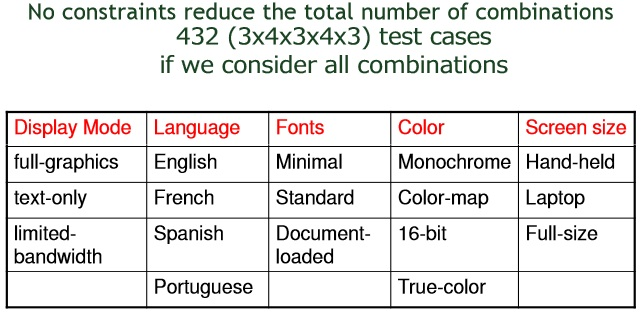
\includegraphics[width=0.7\linewidth]{testingConstraint1.jpg}
	\caption{}
	\label{fig:testingC1}
\end{figure}
\begin{figure}[h!]
	\centering
	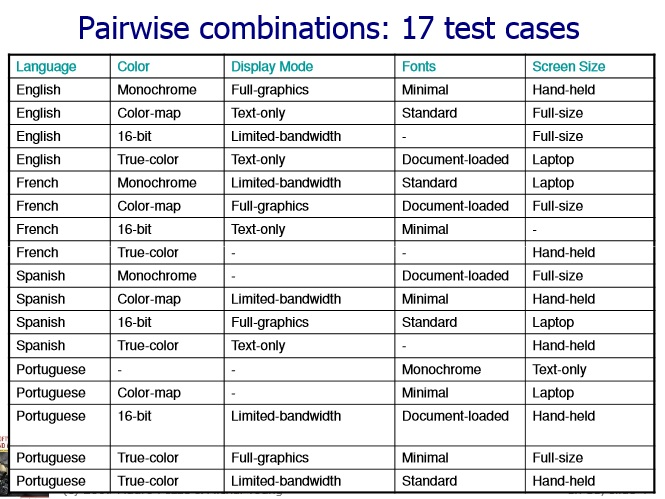
\includegraphics[width=0.7\linewidth]{testingConstraint2.jpg}
	\caption{}
	\label{fig:testingC2}
\end{figure}
\begin{figure}[h!]
	\centering
	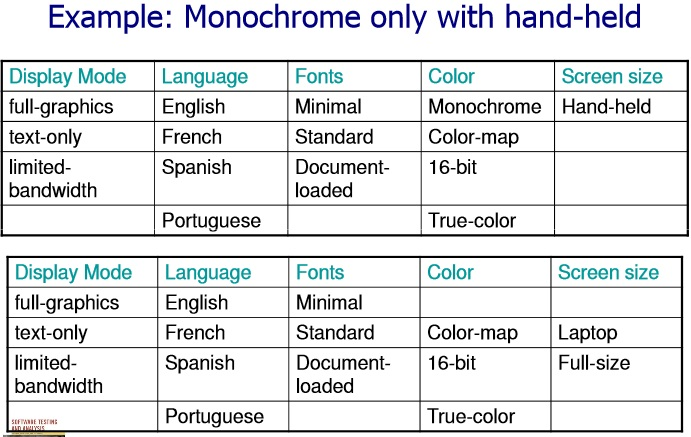
\includegraphics[width=0.7\linewidth]{testingConstraint3.jpg}
	\caption{}
	\label{fig:testingC3}
\end{figure}
\begin{figure}[h!]
	\centering
	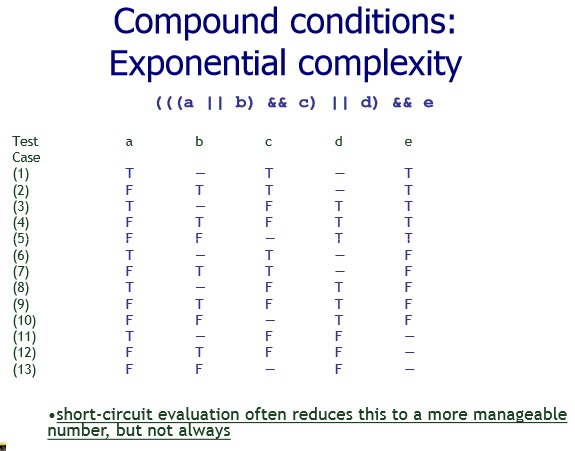
\includegraphics[width=0.7\linewidth]{testingConstraint4.jpg}
	\caption{}
	\label{fig:testingC4}
\end{figure}

\textbf{Modified condition/decision}
\begin{itemize*}
\item Motivation: Effectively test important combinations of conditions, without exponential blowup in test suite size 
\begin{itemize*} 
\item “Important” combinations means: Each basic condition shown to independently affect the outcome of each decision
\end{itemize*}
\item Requires:
\begin{itemize*}
\item For each basic condition C, two test cases,
\item values of all evaluated conditions except C are the same 
\item compound condition as a whole evaluates to true for one and false for the other
\end{itemize*}
\end{itemize*}

\begin{figure}[h!]
	\centering
	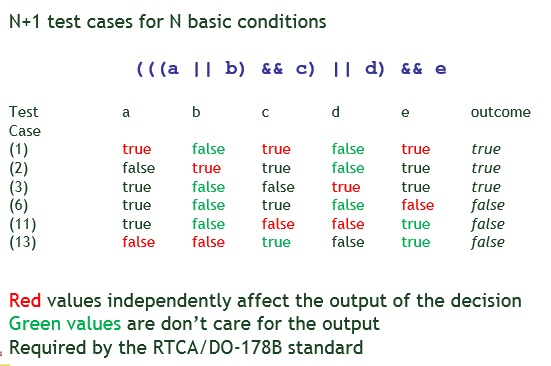
\includegraphics[width=0.7\linewidth]{testingConstraint5.jpg}
	\caption{}
	\label{fig:testingC5}
\end{figure}

\textbf{Comments}
\begin{itemize*}
\item MC/DC is
\begin{itemize*}
\item basic condition coverage (C)
\item branch coverage (DC)
\item plus one additional condition (M): every condition must independently affect the decision's output
\end{itemize*}
\item It is subsumed by compound conditions and subsumes all other criteria discussed so far
– stronger than statement and branch coverage
\item A good balance of thoroughness and test size
(and therefore widely used)
\end{itemize*}

\subsubsection{Mutation Testing}
\begin{itemize*}
\item Evaluation of test suite : What is good test data ?
\item Measure/comparison of test data quality/test methods
\item Improve/increment a test set
\item Evaluation by large number of mutants: small modifications applied to IUT
\item Try to make test suite that detects all mutants
\item If test suite eliminates all mutants then IUT is likely correct (empirical evidence) else extend test suite to eliminate more mutants
\item Iterative process until (almost) all mutants have been killed
\end{itemize*}


\textbf{Assumptions :}
\begin{itemize*}
\item Competent programmer hypothesis: programmers write programs that are (almost) correct
\item Coupling effect : if small faults are detected then also complex faults are
\item Mutant operators : small faults can be described as small modifications of the program by a set of predefined mutant operators
\begin{itemize*}
\item x $\rightarrow$ y,  $\geq \rightarrow > $, $ < \rightarrow <>$, + $\rightarrow$ -
\end{itemize*}
\item Test oracle : criterion to check correctness of output
\item Complexity
	\begin{itemize*}
		\item  number of mutants $\approx O(loc^2)$
	\end{itemize*}
\item Detection of equivalent mutants (testing equivalence on program-level).
\item Useful for test suite quality determination, test selection (remove redundant tests), and experimental comparison of methods
\item Tool support required
\item Optimizations possible:
\begin{itemize*}
\item systematic test generation from living mutants
\item symbolic methods : mutation templates
\item approximations
\end{itemize*}
\end{itemize*}